\chapter{各扰动场基本特征}

我们施加扰动场是为了使得等离子体在有理面被激发出磁岛链,当两个有理面上的磁岛链相互接触之后进一步发展,可产生随机场以削弱边界局域模。磁岛的宽度取决于扰动场在其有理面上和螺旋度相共振的分量,下面我们对各扰动场先分析基本特征,以便于之后的综合优化。

程序内各扰动场的网格分布由毕奥-萨伐尔定律计算线圈或电流丝中的线电流给出,
\begin{equation}\vec{B}(P)=\frac{\mu_{0}}{4 \pi} \sum_{i=1}^{n_{coils}}\left(\oint_{c o i l_{i}} \frac{I_{i} d \vect{r} \times \vect{r}}{r^{3}}.\right)\end{equation}
沿线圈 $\mathrm{d} \vect{r}$ 做积分,其中 $\mu_0$ 是真空磁导率, $I_i$ 是线圈中通过的电流数。$\vect{r}$ 表示点 $\vect{P}$ 和线圈上点之间的位矢。当我们讨论托卡马克这类环向对称的装置来说,通常 $\vect{B}^R\equiv \vect{B}\cdot \vect{e}_R$、$\vect{B}^Z\equiv \vect{B}\cdot \vect{e}_Z$ 表示极向分量,环向分量则用 $\vect{B}^\varphi \equiv \vect{B}\cdot \vect{e}_\varphi$ 表示。


\section{扰动场谱分析理论}
我们首先确定工作在平衡场的本征坐标下 $\left(s, \theta^{*}, \varphi\right),$ 其中 $s \equiv \psi^{1 / 2}(\psi$ 是归一化极向磁通,充当径向坐标,磁面被定义为 $s$ 为常数的一个闭合面,特别的 $s=0$ 代表磁轴而 $s=1$ 表示等离子体边界, 另外取$\theta$ 到 $\theta^{*}(\theta)$ 的非线性变换使得磁力线在 $\left(s, \theta^{*}, \varphi\right)$ 坐标系统中是直线,即 $\left.\frac{d \varphi}{d \theta^{*}}\right|_{F L}=q$,下标 FL 表示取沿着磁力线方向的导数,接着定义三个方向的磁场分量:
% We work in the intrinsic equilibrium coordinates $\left(s, \theta^{*}, \varphi\right),$ where $s \equiv \psi^{1 / 2}(\psi$ being the normalized poloidal magnetic flux, cf. introduction) is used as a radial coordinate (in the $\left(s, \theta^{*}, \varphi\right)$ system of coordinates, a flux surface is defined by $s=c t e,$ in particular $s=0$ for the magnetic axis and $s=1$ for the separatrix $^{1}$ ), and $\theta^{*}$ is such that field lines are straight in the $\left(s, \theta^{*}, \varphi\right)$ system of coordinates:
% where the derivative is taken along a field line. We define:
\begin{equation}
  \begin{aligned}
B^{1} \equiv & \vec{B} \cdot \vec{\nabla} s \\
B^{2} \equiv & \vec{B} \cdot \vec{\nabla} \theta^{*} \\
B^{3} \equiv & \vec{B} \cdot \vec{\nabla} \varphi\\
  \end{aligned}
\label{de:B-comp}
% \tag{B^{i} \text{分量定义}}
\end{equation}

下面我们用磁场环向分量除以径向分量,该量频谱在有理面上的共轭分量最终会出现在磁岛半径计算的表达式中,此后我们对其进行 Fourier 分析找到与其所在有有理面共振的分量。
\begin{equation}
  \tilde{b}^{1} \equiv B^{1} / B^{3}
\end{equation}

% 而垂直磁面的归一化磁扰动分量有下面的表达式:
% and our radial-like normalized magnetic perturbations have the following expression:
% \[
% b^{r} \equiv \frac{b^{1}}{\sqrt{g^{11}}}
% \]

\begin{equation}
  \tilde{b}_{m n}^{1}(s) \equiv \int_{\varphi=0}^{2 \pi} \int_{\theta^{*}=0}^{2 \pi} \tilde{b}^{1}\left(s, \theta^{*}, \varphi\right) e^{-i\left(m \theta^{*}+n \varphi\right)} \frac{d \theta^{*}}{2 \pi} \frac{d \varphi}{2 \pi}
\end{equation}

\begin{equation}
  \tilde{b}^{1}\left(s, \theta^{*}, \varphi\right)=\sum_{m, n=-\infty}^{\infty} \tilde{b}_{m n}^{1}(s) e^{i\left(m \theta^{*}+n \varphi\right)}
\end{equation}

  % 其中 $b^{1} \equiv B^{1} / B_{0}$,$B_{0}$ 是真空中磁轴处环向磁场而 $g^{11} \equiv \vec{\nabla} s \cdot \vec{\nabla} s $。 
  % where $b^{1} \equiv B^{1} / B_{0}(B_{0}$ being the vacuum toroidal magnetic field on the geometrical axis) . and $g^{11} \equiv \vec{\nabla} s \cdot \vec{\nabla} s .$ A poloidal cut of $b^{r}$ produced by the I-coils in even parity configuration is shown in fig. 3.2.
  
\subsection{计算共振分量}
% 3.2 .3 Calculation of the resonant harmonics

下面我们将计算垂直磁面的磁扰动分量在二维磁面上 $(\varphi, \theta^{*})$ 做 Fourier 分析,具体而言我们需要计算 $\tilde{b}^{1} \equiv B^{1} / B^{3}$ 的磁谱。
% Next step consists in calculating the Fourier spectrum of the radial-like magnetic perturbations with respect to the toroidal angle $\varphi$ and intrinsic poloidal angle $\theta^{*} .$ More exactly, one needs to calculate the Fourier spectrum of
因为他是 $\tilde{b}^{1}$ 出现在磁岛宽度表达式中的共振分量。下面定义:
\[
\tilde{b}_{m n}^{1}(s) \equiv \int_{\varphi=0}^{2 \pi} \int_{\theta^{*}=0}^{2 \pi} \tilde{b}^{1}\left(s, \theta^{*}, \varphi\right) e^{-i\left(m \theta^{*}+n \varphi\right)} \frac{d \theta^{*}}{2 \pi} \frac{d \varphi}{2 \pi}
\]
于是:
% so that:
\[
\tilde{b}^{1}\left(s, \theta^{*}, \varphi\right)=\sum_{m, n=-\infty}^{\infty} \tilde{b}_{m n}^{1}(s) e^{i\left(m \theta^{*}+n \varphi\right)}
\]
注意, 因为 $\tilde{b}^{1}$ 为实数,一定有:
$\tilde{b}_{-m,-n}^{1}=\left(\tilde{b}_{m n}^{1}\right)^{*}$
% It should be noticed that, because $\tilde{b}^{1}$ is a real number, we have:


其中星号表示复共轭。由磁面坐标系特征知沿着磁力线,有 $d \varphi=q d \theta^{*},$ 故而 $m \theta^{*}-n \varphi$ 在一条位于有理面 $q=m / n$ 的磁力线上是常数。本文中指有理面 $q=m/n$ 时,$m,n$ 互质,当讨论其谐频时,会用较为明显的 $km/kn$ 表示。注意,该磁面对应的 $\tilde{b}^{1}$ 的磁谱分量不是 $\tilde{b}_{m,n}^{1}$ 和 $\tilde{b}_{-m,-n}^{1}$ 而是 $\tilde{b}_{m,-n}^{1}$ 、 $\tilde{b}_{-m, n}^{1}$ 以及各谐频 $\tilde{b}_{2 m,-2 n}^{1}$ 等。 Eric\cite{nardon_edge_2007} 论文中仅考虑单一环向模数占主导的情况 $n=n_0$,由于本文讨论的多种扰动场磁谱更加复杂,且有其各扰动场之间耦合产生的影响,我们将拓展其在多环向模数下的研究。下面我们在有理面 $q=m/n$ 上将 $\tilde{b}^{1}$ 的共振磁谱分量找出:
% where the star designates the conjugate complex number. Our convention is that, along a field line, we have: $d \varphi=q d \theta^{*},$ so that $m \theta^{*}-n \varphi$ is a constant quantity on a field line located on the $q=m / n$ surface. One should therefore keep in mind that the components of $\tilde{b}^{1}$ that are resonant on such a surface are not $\tilde{b}_{m n}^{1}$ and $\tilde{b}_{-m,-n}^{1}$ but $\tilde{b}_{m,-n}^{1}$ and $\tilde{b}_{-m, n}^{1}$ (and also $\tilde{b}_{2 m,-2 n}^{1}$ etc.). We will often be considering cases where one toroidal harmonic $\left(n_{0}\right)$ is dominant over the others. For instance, in the case of the DIII-D I-coils, the $n_{0}=3$ harmonic dominates. Then, the resonant surfaces which we will consider are those of the type $q=m / n_{0} .$ Let us express the resonant part of $\tilde{b}^{1}$ on such a surface:
\begin{equation}
  \label{eq:resonant-part-series}
\begin{aligned}
  \left(\tilde{b}^{1}\right)_{r e s} &=\sum_{k=1}^{\infty} \tilde{b}_{km,-kn}^{1} e^{i\left(km \theta^{*}-kn \varphi\right)}+ \sum_{k=1}^{\infty}  \tilde{b}_{-km, kn}^{1} e^{i\left(-km \theta^{*}+kn \varphi\right)} \\
  &= \sum_{k=1}^{\infty}  2 \Re\left(\tilde{b}_{km,-kn}^{1} e^{i\left(km \theta^{*}-kn \varphi\right)}\right) \\
  &=\sum_{k=1}^{\infty}  2\left|\tilde{b}_{km,-kn}^{1}\right| \sin \left(km \theta^{*}-kn\varphi + \angle\tilde{b}_{km,-kn}^{1} + \pi/2 \right)\\
  &=\sum_{k=1}^{\infty}  2\left|\tilde{b}_{km,-kn}^{1}\right| \sin \left(km\chi + \angle\tilde{b}_{km,-kn}^{1} + \pi/2 \right)\qquad \chi = \theta^*- \frac{n}{m} \varphi
  \end{aligned}
\end{equation}
其中 $\Re$ 表示取复数的实部、$\angle $ 表示取复数的角度。 对于基频占主导的扰动场,可以仿照 Eric \cite{nardon_edge_2007} 的定义
\begin{equation}
  \tilde{b}_{res}^{1} \equiv 2\left|\tilde{b}_{m,-n_{0}}^{1}\right|
\end{equation}
以方便计算磁岛半径,但于谐频分量也需考虑的情况,上述定义不再方便。


\subsection{估计磁岛宽度及 Chirikov 参数}
用 $s$ 表达的 $q=m / n$ 产生的磁岛半宽度,标记为 $\delta_{q=m / n}$,扰动场在基频 $m/n$ 模式占主导时可以引用 Eric \cite{nardon_edge_2007} 的结果:
% The islands half-widths in terms of $s$ on the $q=m / n$ surface, denoted $\delta_{q=m / n},$ is estimated using the following expression, which is derived in appendix $\mathrm{A}$
\begin{equation}
  \delta_{q=m / n}=\left(\frac{4 q^{2} \tilde{b}_{r e s}^{1}}{q^{\prime} m}\right)^{1 / 2}
\end{equation}

其中 $q^{\prime} \equiv d q / d s$ 是磁剪切。对谐频成分不可忽略的情况则我们需要求该无穷三角函数序列的最大值、最小值,其解析求解是不平凡的。即使截断了有限项也难以求其最值解析表达式,本文中取数值结果最值即可,
\begin{equation}
  \Sigma_{res} = \max_{\chi\in [0,2\pi)} - \min_{\chi\in [0,2\pi)}\sum_{k=1}^{\infty} \frac{2\left|\tilde{b}_{km,-kn}^{1}\right|}{km}   \cos \left(km\chi + \angle\tilde{b}_{km,-kn}^{1} + \pi/2 \right)
\end{equation}

其推导过程见下,

\begin{equation}
  \chi = \theta^*- \frac{n}{m} \varphi
\end{equation}

则沿磁力线求导有,
\begin{equation}\left.\frac{d \chi}{d \varphi}\right|_{F L}=\frac{B^{2}}{B^{3}}-\frac{n}{m}\end{equation}

在有理面 $q=m/n$ 上,位于半径 $s=s_0$ 处,取以下逼近,
\begin{equation}\begin{aligned}
  \frac{B^{2}}{B^{3}} &=\frac{1}{q} \\
  & \simeq \frac{1}{\frac{m}{n}+\bar{s} q^{\prime}} \\
  & \simeq \frac{n}{m}\left(1-\frac{n}{m} \bar{s} q^{\prime}\right)
  \end{aligned}\end{equation}

其中 $\bar{s} \equiv s-s_{0}$ 而磁剪切取常数 $\left.q^{\prime} \equiv \frac{d q}{d s}\right|_{s=s_{0}} .$ 上述两式结合有:
  \[
  \begin{aligned}
  \left.\frac{d \chi}{d \varphi}\right|_{F L} & \simeq-\left(\frac{n}{m}\right)^{2} \bar{s} q^{\prime} \\
  & \simeq-q^{-2} \bar{s} q^{\prime}
  \end{aligned}
  \]

  \begin{equation}\begin{aligned}
    \left.\frac{d \bar{s}}{d \chi}\right|_{F L} &=\left.\left.\frac{d \bar{s}}{d \varphi}\right|_{F L} \cdot \frac{d \varphi}{d \chi}\right|_{F L} \\
    &=\left.\frac{d s}{d \varphi}\right|_{F L} \cdot\left(\left.\frac{d \chi}{d \varphi}\right|_{F L}\right)^{-1} \\
    & \simeq-\frac{B^{1}}{B^{3}} \frac{q^{2}}{\bar{s} q^{\prime}}
    \end{aligned}\end{equation}

其中 $\frac{B^{1}}{B^{3}}$ 仅取共振部分,有
    $$\left(\frac{B^{1}}{B^{3}}\right)_{r e s}= \left(\tilde{b}^1\right)_{r e s}=\sum_{k=1}^{\infty}  2\left|\tilde{b}_{km,-kn}^{1}\right| \sin \left(km\chi + \angle\tilde{b}_{km,-kn}^{1} + \pi/2 \right)$$

则有
\begin{equation}
  \bar{s} d \bar{s} \simeq-\frac{q^{2} }{q^{\prime}} \left( \sum_{k=1}^{\infty}  2\left|\tilde{b}_{km,-kn}^{1}\right| \sin \left(km\chi + \angle\tilde{b}_{km,-kn}^{1} + \pi/2 \right)\right)d \chi 
\end{equation}

\begin{equation}
  \frac{1}{2} d\left(\bar{s}^{2}\right) \simeq \frac{q^{2}}{q^{\prime} } d[\sum_{k=1}^{\infty} \frac{2\left|\tilde{b}_{km,-kn}^{1}\right|}{k m}  \cos \left(km\chi + \angle\tilde{b}_{km,-kn}^{1} + \pi/2 \right)]
\end{equation}


\begin{equation}\bar{s}^{2} \simeq \frac{2 q^{2} }{q^{\prime} }[\sum_{k=1}^{\infty} \frac{2\left|\tilde{b}_{km,-kn}^{1}\right|}{k m}  \cos \left(km\chi + \angle\tilde{b}_{km,-kn}^{1} + \pi/2 \right) + C]\end{equation}

以上取不同的积分常数会得到对应的磁岛链,其磁岛链分界线对应着刚好存在有限个极小点为零的积分常数 $C$,则磁岛半宽度依赖于峰峰值

\begin{equation}
  \delta_{q=m / n}=\left(\frac{2 q^{2} \Sigma_{res}}{q^{\prime} }\right)^{1 / 2}
\end{equation}

Chirikov 参数在 $q_1$ 和 $q_2$ 有理面之间记为 $\sigma_{C h i r}^{q_1, q_2}$ 最终计算为:
% where $q^{\prime} \equiv d q / d s$ is the magnetic shear. Fig. 3.5 shows the $q$ profile for DIII-D shot 125913 together with symbolic islands represented by horizontal bars of half-widths $\delta_{q=m / n}$ produced by the I-coils fed with $4 \mathrm{kAt}$, for both even and odd parity configurations. The Chirikov parameter in-between the $q=m / n$ and $q=(m+1) / n$ surfaces, denoted $\sigma_{C h i r}^{m, m+}$ is finally calculated as:
\[
\sigma_{C h i r}^{q_1, q_2} \equiv \frac{\delta_{q=q_1}+\delta_{q=q_2}}{\Delta_{q_1, q_2}}
\]
其中 $\Delta_{q_1, q_2}$ 表示两有理面之间的径向距离 (用归一化径向坐标 $s$ 表示) 。
% where $\Delta_{q_1, q_2}$ designates the radial distance (in terms of $s$ ) between the $q=m / n$ and the $q=(m+1) / n$ surfaces, which can be approximated as:


\section{ERGOS}

ERGOS 程序是 Fortran、Matlab 语言编写的三维扰动场分析程序,它通过对 EFIT 产生的平衡场数据进行处理,构建基于平衡磁场的磁面坐标系,在磁面坐标系上对扰动场进行分解并对垂直磁面的分量进行 Fourier 分析,从而估计扰动场的磁谱和磁谱共振部分在有理面上激发的磁岛宽度;另外 ERGOS 还带有通过磁力线追踪对扰动场拓扑进行分析的工具。ERGOS 最初用于 ITER 的 ELMs 抑制线圈设计,后来在各大装置上先后被用来分析 RMP 线圈产生的共振磁扰动,如 JET、MAST、COMPASS-D 等。

基于以下几点对 ERGOS 的考虑,本文研究过程中对其进行了完全的重构。

\begin{enumerate}[(i)]
  \item ERGOS 计算 Chrikov 参数的变量依赖于给定的 $n$, 在没有主导的 $n$ 的扰动场中(如高 m 线圈)或者用户给定的 $n$ 不准确的情况下,Chrikov 参数可能是不准确的。
  \item 函数输入输出变量直接储存于 Matlab 环境中,不太便于函数调用以对多扰动场进行协同分析。
  \item ERGOS 原本对每个线圈计算场都要单独写程序。改写后统一数据接口,可以直接处理工程 Excel 表的线圈线型几何数据。
\end{enumerate}


虽然将 ERGOS 重新构造一遍所花的时间较多,但可以避免 Matlab 所需要的版权费用,且当前中美形势紧张。重构后的 ERGOS 具备许多更加智能且方便快捷的功能,可以更好地作为科研的基础工具。

各扰动场在对应的场源为 \SI{1}{\kilo\ampere t} 时的扰动场被保存为标准场数据文件。标记各扰动场源正方向,\textit{(1) RMP 线圈 / 低 n 线圈} 产生的 $B^1$ 在作用的核心区为正即为正  \textit{(2) 高 m 线圈} 确定主要工作模式 $B^1$ 从上至下是 -,+,-,+ 分布,次要工作模式是 -,+,-; \textit{(3) 螺旋电流丝} FLT 电流沿磁场方向即为正方向。


  
    


  


\section{磁谱特征分析}

\begin{figure}[htbp]
  \centering%
      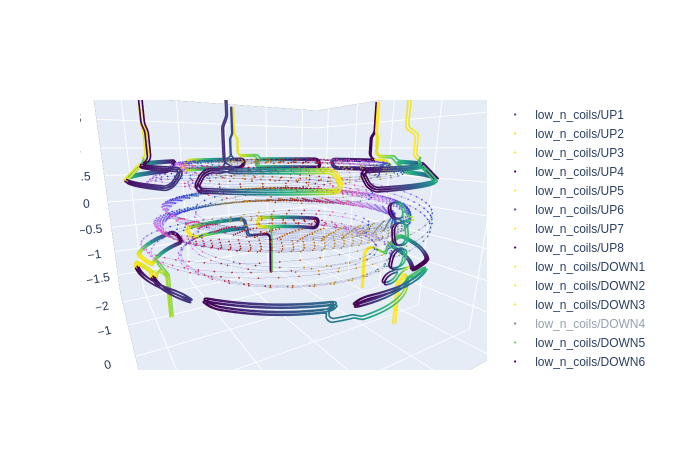
\includegraphics[width=0.55\columnwidth]{coil_collab.png}
      \caption{涉及到的扰动场源的几何形状,图中上下两排环向排列的线圈为低 n 线圈,在图右侧的低场侧分布着四个上下排列的线圈是高 m 线圈,螺旋电流丝在图中呈螺旋形缠绕的中间的等离子体。}
      \label{fig:current-topo}
\end{figure}

本文中涉及的扰动场形状、功能设计及产生原因不尽相同,在模拟中涉及到的它们的线电流源形状如图 \ref{fig:current-topo} 所示。

\subsection{低 n 线圈}
低 n 线圈原本被称为 RMP 线圈,因为起初产生强共振分量的扰动场仅有此种手段,本文中我们根据其特征称它为低 n 线圈,它是图 \ref{fig:current-topo} 中上下沿各八个环向排列的鞍形线圈。


\begin{figure}[htbp]
  \centering%
  \begin{subfigure}{0.45\textwidth}
    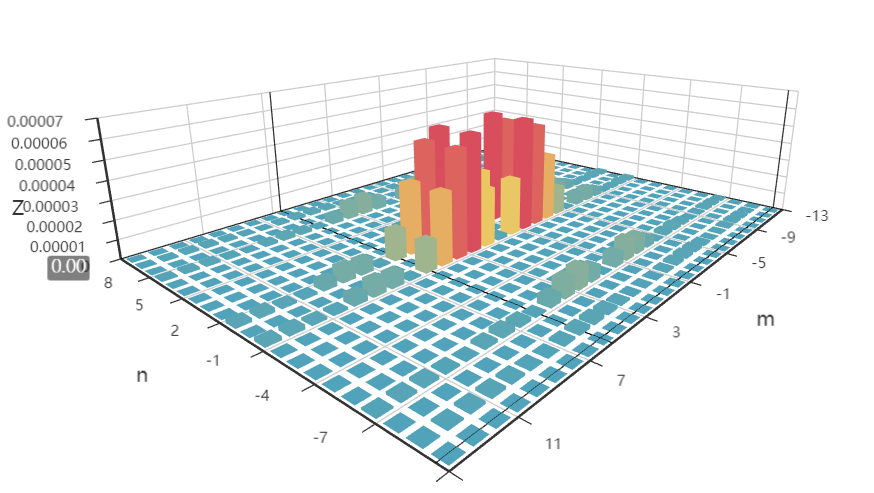
\includegraphics[height=3.7cm]{spectrum/low_n_odd_n_is_1_s_is_09.png}
    \caption{Odd 奇连接,主导模式 $n=1$}
  \end{subfigure}%
  % \hspace{4em}%
  \begin{subfigure}{0.45\textwidth}
    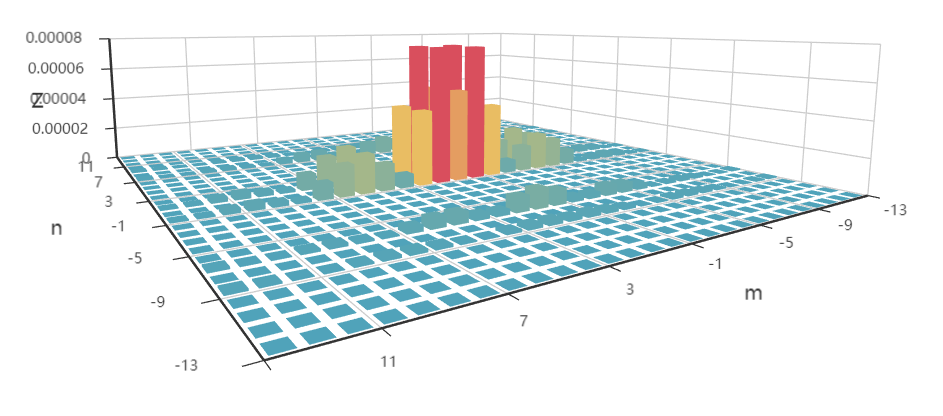
\includegraphics[height=3.7cm]{spectrum/low_n_even_n_is_1_s_is_09.png}
    \caption{Even 偶连接,主导模式 $n=1$}
  \end{subfigure}
  
  \begin{subfigure}{0.45\textwidth}
    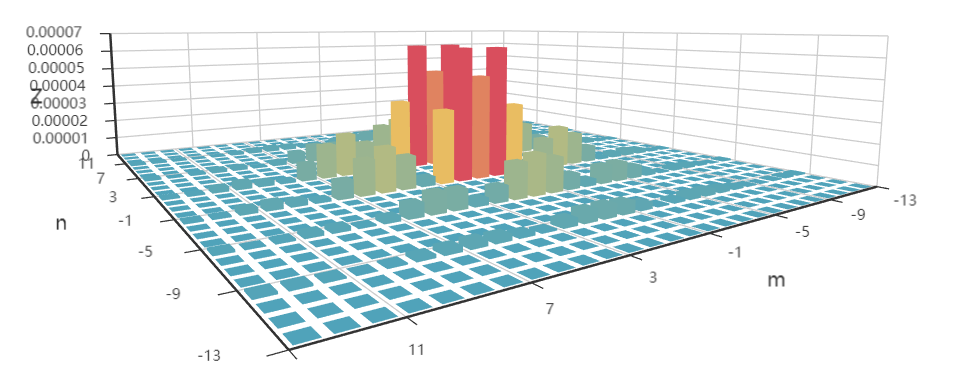
\includegraphics[height=3.7cm]{spectrum/low_n_even_n_is_2_s_is_09.png}
    \caption{Odd 奇连接,主导模式 $n=2$}
  \end{subfigure}
  \begin{subfigure}{0.45\textwidth}
    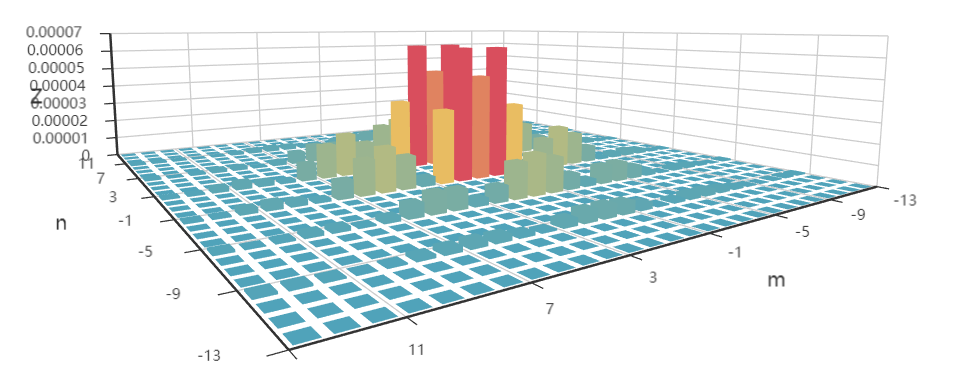
\includegraphics[height=3.7cm]{spectrum/low_n_even_n_is_2_s_is_09.png}
    \caption{Even 偶连接,主导模式 $n=2$}
  \end{subfigure}
  \caption{低 n 线圈作用下于 $s=0.9$ 处的磁扰动谱 $\tilde{b}^1_{mn}$}
  \label{fig:lown-spectrum-subfig}
\end{figure}


从图 \ref{fig:lown_current} 中可以看出,低 n 线圈有较清晰的谐频特征。若设置主导模数为 $n_0$,则仅在 $n=kn_0$ 处有较强的 $|\tilde{b}^1_{mn}|$,见图 \ref{fig:lown-spectrum-subfig}。

\subsection{高 m 线圈}

高 m 线圈被设计用来探究有高 m,宽 n 特征的扰动场对等离子体的影响,并研究这种强局域性的磁扰动会否对等离子体边界的稳定性造成影响。其与目前RMP线圈系统潜在的协同作用在本文中进行初步调研。



\begin{figure}[htbp]
  \centering%
  % \hspace{4em}%
  \begin{subfigure}{0.65\textwidth}
      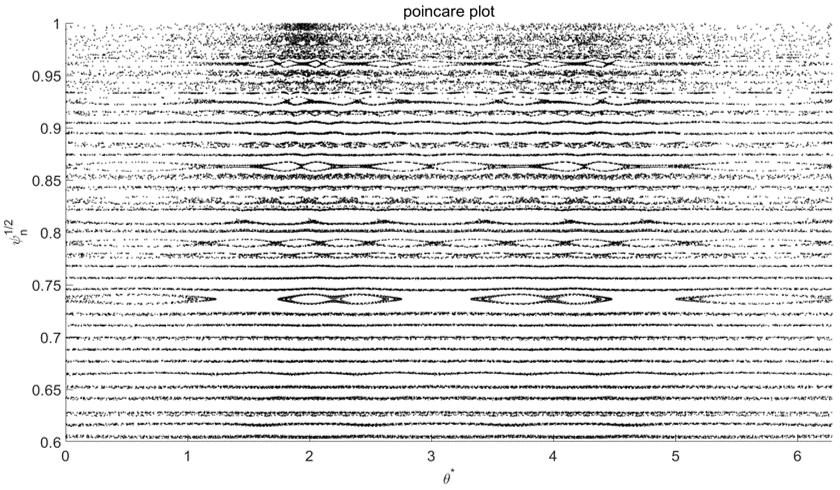
\includegraphics[height=6.2cm]{highm/stretched_poincare_primary_state.png}
      \caption{高 $m$ 线圈主要工作模式下展开的 \Poincare 图}
  \end{subfigure}
  % \hspace{4em}%
  \begin{subfigure}{0.7\textwidth}
      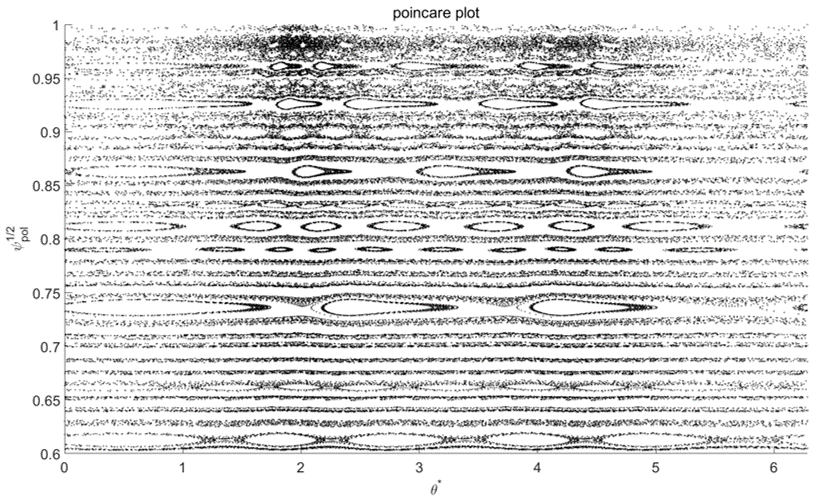
\includegraphics[height=6.6cm]{highm/stretched_poincare_secondary_state.png}
      \caption{高 $m$ 线圈次要工作模式下展开的 \Poincare 图}
  \end{subfigure}
  \caption{高 $m$ 线圈作用下的 \Poincare 图,次要工作模式下的磁扰动情况较主要模式更深,源自等离子体所张华祥研究员\cite{zhang_highm} }
  \label{fig:highm-stretched-poincare}
\end{figure}


\subsection{螺旋电流丝}

螺旋电流丝由于在刮削层中沿磁力线产生,所以其产生的扰动场与等离子体边界附近的有理面相贴合,其对边界随机场的产生有很大的贡献。观察下图 \ref{fig:HCFs-b1-tilde} ,发现螺旋电流丝的磁谱在沿着磁面螺旋度的方向上有着较高的共振分量,其磁谱脊线不沿着 m 轴或 n 轴,而是稍微与坐标轴有一定的斜率,很好地贴合了边界的螺旋度。

\begin{figure}[htbp]
  \centering%
  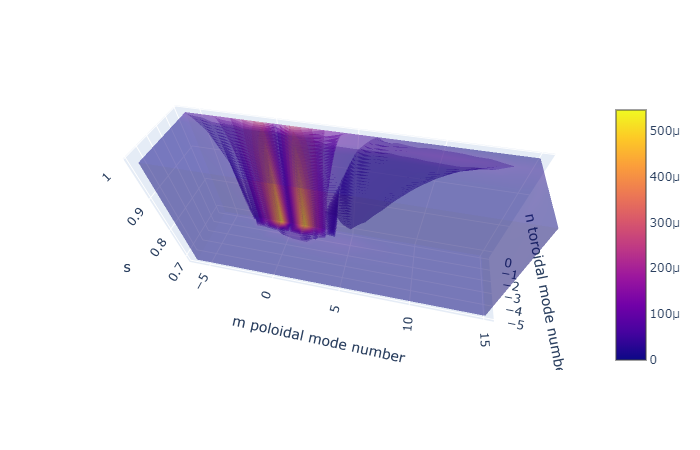
\includegraphics[width=1.00\columnwidth]{spectrum/HCFs_uniform_volume.png}
  \caption{螺旋电流丝总电流大小为 1kA 时的磁谱 $|\tilde{b}^1_{mn}|$ }
  \label{fig:HCFs-b1-tilde}
\end{figure}
